\input{header.tex}

\title{Guest Lecture on Data Parallel Programming}
\date{\today{} at \currenttime{}}
\author{Troels Henriksen}

\usepackage{futhark}

\lstset{language=futhark,showlines=true}

\begin{document}

\maketitle

\begin{frame}
  \frametitle{Who am I}

  \begin{itemize}
  \item Researcher at the University of Copenhagen.
  \item I work on
    \begin{itemize}
    \item Data parallel programming
    \item Data parallel algorithms
    \item Programming language design and implementation
    \item High performance computing, particularly on GPUs
    \item Compiler optimisations
    \item Various other programming language topics
    \end{itemize}
  \item My main \emph{practical} research artifact is the \emph{Futhark
      programming language}.
  \end{itemize}

\end{frame}

\begin{frame}
  \frametitle{Two kinds of parallelism}

  \begin{block}{Task parallelism}
    Simultaneously doing different things to different data
    \begin{itemize}
    \item E.g., multithreading, message passing.
    \item Usually nondeterministic.
    \end{itemize}
  \end{block}

  \begin{block}{Data parallelism}
    Simultaneously doing \emph{the same thing} to different data.
    \begin{itemize}
    \item Bulk operations on entire collections of data.
    \item E.g., \texttt{map}!
    \item Usually deterministic.
    \end{itemize}
  \end{block}
\end{frame}

\begin{frame}
  \frametitle{You already know data parallel programming!}

  \pause\bigskip

  If \texttt{x} and \texttt{y} are vectors, then \texttt{x + y} is a
  data parallel operation.

  \pause\bigskip

  \begin{itemize}
  \item NumPy, R, Matlab, Julia, SQL are all data parallel models.
  \item Completely sequential and deterministic semantics.
  \item Parallel \textit{execution} straightforward.
  \item \textbf{Distinguish between parallel execution and parallel potential.}
    \begin{itemize}
    \item Implementations can always be parallelised as long as the
      code is written in a parallel style.
    \end{itemize}
  \end{itemize}

  \textbf{We will make this notion precise in a bit.}
\end{frame}

\begin{frame}{Data parallel vocabulary}

  \textbf{Data parallel programming involves expressing operations on
    \emph{entire data collections} at a time---in our case, arrays.}

  \begin{block}{\texttt{map}}
    \[
      \texttt{map}~f~[x_{0}, \ldots, x_{n-1}] = [f~x_{0}, \ldots, f~x_{n-1}]
    \]
  \end{block}

  \begin{block}{\texttt{sum}}
    \[
      \texttt{sum}~[x_{0}, \ldots, x_{n-1}] = x_{0} + \ldots + x_{n-1}
    \]
  \end{block}
\end{frame}

\begin{frame}[fragile]
  \frametitle{Summation, sequentially}

\begin{lstlisting}
def sum (xs: []i32) =
  loop y = 0 for i < length xs do
    y + xs[i]
\end{lstlisting}

  Is this good?

\end{frame}

\begin{frame}[fragile]
  \frametitle{Summation, in parallel}

\begin{lstlisting}
def sum (xs: []i32) =
  loop ys = xs while length ys > 1 do
    let ys_first = take (length ys / 2) ys
    let ys_last  = drop (length ys / 2) ys
    in map2 (+) ys_first ys_last
\end{lstlisting}

  \pause \small
  \begin{tabular}{lcr}
    \texttt{ys} & = &        \texttt{[1, 2, 3, 4, 5, 6, 7, 8]} \\
    \texttt{ys\_first} & = & \texttt{[1, 2, ~3, ~4]} \\
    \texttt{ys\_last} & = &  \texttt{[5, 6, ~7, ~8]} \\\hline
    \texttt{ys} & = &        \texttt{[6, 8, 10, 12]} \\
    \texttt{ys\_first} & = & \texttt{[~6, ~8]} \\
    \texttt{ys\_last} & = &  \texttt{[10, 12]} \\\hline
    \texttt{ys} & = &        \texttt{[16, 20]} \\
    \texttt{ys\_first} & = & \texttt{[16]} \\
    \texttt{ys\_last} & = &  \texttt{[20]} \\\hline
    \texttt{ys} & = & \texttt{[36]} \\
  \end{tabular}

\end{frame}

\begin{frame}[fragile]
  \frametitle{Comparison}

  \begin{columns}
    \begin{column}[t]{.45\textwidth}
\begin{lstlisting}
def sum (xs: []i32) =
  loop y = 0 for i < length xs do
    y + xs[i]


\end{lstlisting}

      $O(n)$ work, but sequential.

    \end{column}
    \begin{column}[t]{.59\textwidth}
\begin{lstlisting}
def sum (xs: []i32) =
  loop ys = xs while length ys > 1 do
    let ys_first = take (length ys / 2) ys
    let ys_last  = drop (length ys / 2) ys
    in map2 (+) ys_first ys_last
\end{lstlisting}

      $O(n)$ work, but parallel.

    \end{column}

  \end{columns}

  \bigskip
  \textbf{We need a framework in which we can be precise about why the parallel
    version is better.}

\end{frame}

\begin{frame}
  \frametitle{Computation DAG for sequential \texttt{sum}}

  \begin{center}
  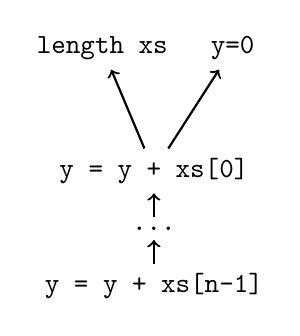
\begin{tikzpicture}
    \node (1a) {\texttt{length xs}};
    \node (1b) [right = 0.3cm,at=(1a.east)]  {\texttt{y=0}};
    \node (2) [below = 1cm,at=(1b.south), xshift=-1cm]  {\texttt{y = y + xs[0]}};
    \node (3) [below = 0.3cm,at=(2.south)]  {\texttt{...}};
    \node (4) [below = 0.3cm,at=(3.south)]  {\texttt{y = y + xs[n-1]}};

    \path[draw,thick,<-]
    (1a) edge node {} (2)
    (1b) edge node {} (2)
    (2) edge node {} (3)
    (3) edge node {} (4)
    ;
\end{tikzpicture}
  \end{center}

      \begin{itemize}
      \item Total count of nodes is the \textit{work}, $W(p)$.
      \item Length of longest path from a leaf to the root is the
        \textit{span}.
      \item \textbf{With an infinite number of processors, if a program $p$ has
          span $k$, written $S(p) = k$, the program can execute in $O(k)$
          time.}
      \item Here, $W(p) = O(n)$, $S(p) = O(n)$.
     \end{itemize}

\end{frame}

\begin{frame}
  \frametitle{Computation DAG for parallel \texttt{sum}}

  \begin{center}
  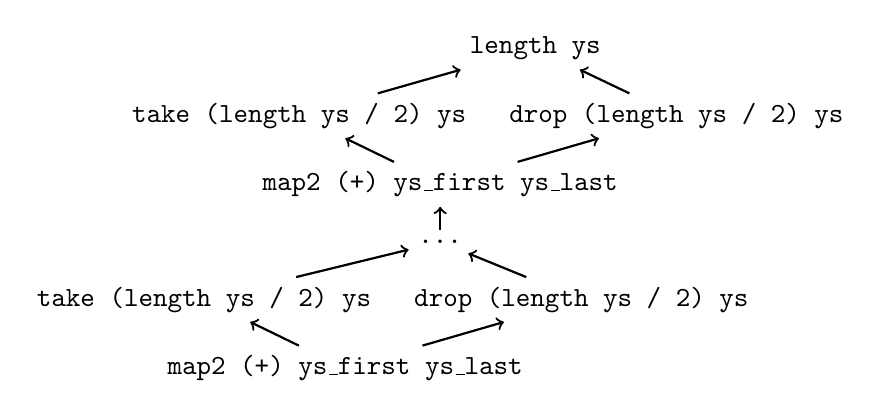
\begin{tikzpicture}
    \node (1) {\texttt{length ys}};
    \node (2a) [below = 0.3cm,at=(1.south), xshift=-3cm]  {\texttt{take (length ys / 2) ys}};
    \node (2b) [right = 0.3cm,at=(2a.east)]  {\texttt{drop (length ys / 2) ys}};
    \node (3) [below = 0.3cm,at=(2b.south), xshift=-3cm]  {\texttt{map2 (+) ys\_first ys\_last}};
    \node (4) [below = 0.3cm,at=(3.south)]  {\texttt{...}};
    \node (5a) [below = 0.3cm,at=(4.south), xshift=-3cm]  {\texttt{take (length ys / 2) ys}};
    \node (5b) [right = 0.3cm,at=(5a.east)]  {\texttt{drop (length ys / 2) ys}};
    \node (6) [below = 0.3cm,at=(5b.south), xshift=-3cm]  {\texttt{map2 (+) ys\_first ys\_last}};

    \path[draw,thick,<-]
    (1) edge node {} (2a)
    (1) edge node {} (2b)
    (2a) edge node {} (3)
    (2b) edge node {} (3)
    (3) edge node {} (4)
    (4) edge node {} (5a)
    (4) edge node {} (5b)
    (5a) edge node {} (6)
    (5b) edge node {} (6)
    ;
  \end{tikzpicture}

\bigskip

  \textbf{What is the work and span complexity?}

  \end{center}

  \pause

$W(p) = O(n) \quad\quad S(p) = O(\log_{2} n)$

\end{frame}

\begin{frame}[fragile]
  \frametitle{Parallel cost model based on work and span}

  \vspace{1ex}

  Instead of giving just a simple cost-model based on the total notion
  of work carried out by a program, we give instead a \emph{refined}
  cost model, which aims at providing both:
  \begin{itemize}
  \item a notion of how much total work ($W$) the program does;
  \item a notion of the \emph{span} ($S$) of the program, specifying the maximum
    depth required by the computation.
  \end{itemize}

\bigskip\textbf{Notice:}

\begin{itemize}
  \item The span is the length of the longest sequence of operations
    that must be performed sequentially due to data dependencies.
  \item With an infinite number of processors, if a program $p$ has
    span $k$, written $S(p) = k$, the program can execute in $O(k)$
    time.
  \end{itemize}
\end{frame}

\begin{frame}
  \frametitle{Brent's Theorem (1974) \hfill (or Lemma, or Law...)}

  Writing $T_{i}$ for the time taken to execute an algorithm on $i$
  processors, Brent's Theorem states that
  \[
    \frac{T_{1}}{p} \leq T_{p} \leq T_{\infty} + \frac{T_{1}}{p}
  \]
  \textbf{Proof sketch:} At level $j$ of the DAG there are $M_{j}$
  independent operations, which can clearly be executed by $p$ processors in time
  \[
    \Bigl\lceil{\frac{M_{j}}{p}}\Bigr\rceil
  \]
  Sum these for each level of the DAG. \qed

  \bigskip

  \begin{block}{Ramification}
    We can simulate an ``infinitely parallel'' machine on a real
    machine at an overhead proportional to the amount of ``missing''
    hardware parallelism.
  \end{block}

\end{frame}

\begin{frame}
  \frametitle{Wait, is that summation correct?}

  In our summation, we changed

\newcommand\redop{\only<1>{+}\only<2->{\oplus}}

  \[
    (((((((x_{0} \redop x_{1}) \redop x_{2}) \redop x_{3}) \redop x_{4}) \redop x_{5}) \redop x_{6}) \redop x_{7})
  \]

  to

  \[
    ((x_{0} \redop x_{4}) \redop (x_{2} \redop x_{6})) \redop ((x_{1} \redop x_{5}) \redop (x_{3} \redop x_{7}))
  \]

  Is that valid?

  \pause

  \bigskip
  What about now?

  \bigskip

  \pause

  \textbf{In general, what must hold for an operator $\oplus$ for such
    a rewrite to be valid?}

\undef\redop

\end{frame}

\begin{frame}
  \frametitle{Commutativity and associativity}

  A binary operator
  $\oplus : \alpha \rightarrow \alpha \rightarrow \alpha$ is said to
  be \textit{commutative} if
  \[
    x \oplus y = y \oplus x
  \]

  \pause

  It is \textit{associative} if
  \[
    x \oplus (y \oplus z) = (x \oplus y) \oplus z
  \]

  If we are a little more clever, we can do a parallel ``sum'' with
  any associative operator.

  \pause

  For convenience, we also tend to require a \textit{neutral element}
  $0_{\oplus}$:
  \[
    x \oplus 0_{\oplus} = 0_{\oplus} \oplus x = x
  \]

\end{frame}

\begin{frame}
  \frametitle{Monoidal summation}

  An associative binary operator
  $\oplus : \alpha \rightarrow \alpha \rightarrow \alpha$ with a
  neutral element $0_{\oplus}$ is called a \textit{monoid} and written
  $(\oplus, 0_{\oplus})$\footnote{A monoid without a neutral element
    is called a \textit{semigroup}}.  Examples:

  \begin{itemize}
  \item $(+, 0)$
  \item $(*, 1)$
  \item $(++, [])$
  \end{itemize}

  \pause

  For any monoid $(\oplus, 0_{\oplus})$ we can construct a function
  \texttt{sum} with \textit{semantics}
  \[
    \texttt{sum}([x_{0}, \ldots, x_{n-1}]) = x_{0} \oplus \ldots \oplus x_{n-1}
  \]
  but which can \textit{operationally} be executed in parallel.

\end{frame}

\begin{frame}
  \frametitle{Monoidal reduction}

  We can abstract the notion of summation into a higher-order function
  typically called \texttt{reduce}:

  \[
    \texttt{reduce} : (\alpha \rightarrow \alpha \rightarrow \alpha) \rightarrow \alpha \rightarrow []\alpha \rightarrow \alpha
  \]

  Then

  \[
    \texttt{sum} = \texttt{reduce}~(+)~0
  \]

  \pause

  \textbf{This is one of the main components of the data parallel vocabulary.}
\end{frame}

\begin{frame}[fragile]
  \frametitle{The Futhark programming language}


  \begin{itemize}
  \item A \emph{functional array language}.
  \item Parallel programming with data-parallel combinators.
  \item Compiles to efficient parallel CPU or GPU code.
  \item Feels like a restricted subset of standard functional languages.
  \end{itemize}

\begin{lstlisting}
def inc2 [n] (xs: [n]i32) : [n]i32 = map (+2) xs

def sum [n] (xs: [n]i32) : i32 = reduce (+) 0 xs

def sumrows [n][m] (xss: [n][m]i32) : [n]i32 = map sum xss
\end{lstlisting}

\end{frame}

\begin{frame}
  \frametitle{Core restrictions}

  \begin{description}
  \item[No irregular arrays:]
    \texttt{[[1], [2,3]]} is a type error.\pause
  \item[No recursive data types:] while recursive \emph{functions} are allowed,
    they are discouraged.\pause
  \item[No side effects:] completely pure.\pause
  \item[Some limitations on first class functions:]\hfill
    \begin{itemize}
    \item Cannot return from \texttt{if}
    \item Cannot be variant in \texttt{loop}
    \item Cannot recurse in polymorphic way.
    \end{itemize}
  \end{description}

  \begin{center}
    Restrictions rooted in desire for good performance, and all checked at
    compile-time.
  \end{center}
\end{frame}

\begin{frame}
  \frametitle{As a language}

  \begin{center}
    \textbf{Not a language for writing applications---a Futhark program is
      compiled to a \emph{library} and then invoked from other languages.}
  \end{center}

  Some material:

  \begin{itemize}
  \item \url{https://futhark-lang.org}
  \item \url{https://futhark-lang.org/docs/prelude/}
  \item \url{https://futhark.readthedocs.io/en/latest/versus-other-languages.html}
  \item \url{https://futhark.readthedocs.io/en/latest/c-api.html}
  \end{itemize}

  But my focus today is general \textbf{data parallel thinking}, so we will see
  only a small part of the language.

\end{frame}

\begin{frame}[fragile]
  \frametitle{\texttt{map} and \texttt{reduce}}

\begin{lstlisting}
-- Work: O(n * W(f))
-- Span: O(1 * S(f))
val map [n] 'a 'b : (f: a -> b) -> [n]a -> [n]b

-- Work: O(n * W(op))
-- Span: O(log(n) * S(op))
val reduce [n] 'a : (op: a -> a -> a) -> a -> [n]a -> a
\end{lstlisting}
  \pause
\begin{lstlisting}
-- Work: O(n)
-- Span: O(1)
val zip [n] 'a 'b : [n]a -> [n]b -> [n](a,b)
\end{lstlisting}
  \pause
\begin{lstlisting}
-- Work: O(n * W(f))
-- Span: O(1 * S(f))
val map2 [n] 'a 'b 'c : (f: a -> b -> c) -> [n]a -> [n]b -> [n]c
\end{lstlisting}

\end{frame}

\begin{frame}[fragile]
  \frametitle{Matrix multiplication}

\begin{lstlisting}
-- Work: O(n*m)
-- Span: O(1)
val transpose [n] [m] 'a : [n][m]a -> [m][n]a
\end{lstlisting}

\pause

\begin{lstlisting}
-- Work: O(n)
-- Span: O(log(n))
def dotprod [n] (x: [n]f64) (y: [n]f64) : f64 =
  reduce (+) 0 (map2 (*) x y)
\end{lstlisting}
\pause
\begin{lstlisting}
def matmul [n] [m] [p] (A: [n][m]f64) (B: [m][p]f64) : [n][p]f64 =
  map (\A_row ->
         map (\B_col ->
                dotprod A_row B_col)
             (transpose B))
      A
\end{lstlisting}
What is the work and span?\pause
\hfill $W=O(n*p*m), S=O(log(m))$.
\end{frame}

\begin{frame}[fragile]
  \frametitle{Scan}
\begin{lstlisting}
-- Work: O(n * W(op))
-- Span: O(log(n) * S(op))
val scan [n] 'a : (op: a -> a -> a) -> a -> [n]a -> [n]a
\end{lstlisting}
  \emph{Semantically}, a scan is the reduce of all prefixes of an array.
\begin{lstlisting}
scan op ne xs = [reduce op ne xs[:1],
                 reduce op ne xs[:2],
                 ...,
                 reduce op ne xs[:n]]
\end{lstlisting}
  \emph{In practice} it is implemented more efficiently.

  \begin{block}{Example of \texttt{scan}}
\begin{lstlisting}
> scan (+) 0 [1,2,3,4,5]
[1, 3, 6, 10, 15]
\end{lstlisting}
  \end{block}
\end{frame}

\begin{frame}[fragile]
  \frametitle{Filtering}

  Suppose we wish to remove negative elements from the list

\begin{lstlisting}
let as = [-1, 2, -3, 4, 5, -6]
\end{lstlisting}

\pause

  For each element, see if we want to keep it:

\begin{lstlisting}
let keep = map (\a -> if a >= 0 then 1 else 0) as
-- [ 0, 1, 0, 1, 1, 0]
\end{lstlisting}

\pause

\begin{lstlisting}
let offsets1 = scan (+) 0 keep
-- [ 0, 1, 1, 2, 3, 3]
\end{lstlisting}

\pause

\begin{lstlisting}
let offsets = map (\x -> x - 1) offsets1
-- [-1, 0, 0, 1, 2, 2]
\end{lstlisting}

\pause

\texttt{offsets[i]} now indicates position in filtered list if
\texttt{keep[i] == 1}.

\end{frame}

\begin{frame}[fragile]
  \frametitle{\texttt{scatter}}

  \texttt{scatter xs is vs} computes equivalent of the imperative
  pseudocode

\begin{lstlisting}[language=Fortran]
for j < n:
  xs[is[j]] = vs[j]
\end{lstlisting}

  \begin{itemize}
  \item Out-of-bound writes are ignored.
  \item Writing different values to same index is
    \textit{undefined}.\footnote{\texttt{reduce\_by\_index} handles conflicts with provided operator.}
  \item Work $O(n)$, span $O(1)$.
  \end{itemize}

  \bigskip
  \textbf{Just what we need for filtering!}

  \pause

\begin{lstlisting}
scatter (replicate (last offsets1) 0)
        (map2 (\i k -> if k == 1 then i else -1)
              offsets keep)
        as
\end{lstlisting}

\end{frame}

\begin{frame}[fragile]
  \frametitle{Implementing a polymorphic \texttt{filter}}

\begin{lstlisting}
def filter [n] 'a (p: a -> bool) (as: [n]a): ?[m].[m]a =
  let keep = map (\a -> if p a then 1 else 0) as
  let offsets1 = scan (+) 0 keep
  let offsets = map (\x -> x - 1) offsets1
  let num_to_keep = n == 0 || last offsets1 == 0
  in scatter (copy (take num_to_keep a))
             (map2 (\i k -> if k == 1
                            then i
                            else -1)
                   offsets keep)
             as
\end{lstlisting}

  The \texttt{copy} is because \texttt{scatter} \emph{consumes} its first argument.

\end{frame}

\begin{frame}[fragile]
  \frametitle{Working with irregular arrays}

  \begin{center}
    \textbf{Forbidden in Futhark: \texttt{[[1], [2,3], [4,5,6]]}}
  \end{center}

  We can still work with such values by \emph{encoding} them in ways that are
  allowed.\pause

  We represent irregular arrays as a pair of two vectors of the same size.
  \begin{description}
  \item[Value vector:] one-dimensional vector of values, e.g.\hfill\\
    \texttt{[1,2,3,4,5,6]}
    \item[Boolean vector:] denotes when a new subarray begins, e.g.\hfill\\
      \texttt{[true, true, false, true, false, false]}
  \end{description}

  We can then define ``segmented operations'' on this encoding---a big topic,
  but we will look at one example.

\end{frame}

\begin{frame}[fragile]
  \frametitle{Segmented scans}
\begin{lstlisting}
val segscan [n] 't
   :  (op: t -> t -> t) -> (ne: t)
   -> (fs: [n]bool) -> (vs: [n]t)
   -> [n]t
\end{lstlisting}

\texttt{true} starts a segment and \texttt{false} continues a segment.

\begin{block}{Example}

\begin{lstlisting}
segscan (+) 0
  [true, false, true, false, false, true]
  [0, 1, 2, 3, 4, 5]
== scan (+) 0 [0,1] ++
   scan (+) 0 [2,3,4] ++
   scan (+) 0 [5]
== [0, 1, 2, 5, 9, 5]
\end{lstlisting}
\end{block}

\end{frame}

\begin{frame}[fragile]
  \frametitle{Implementation of \texttt{segscan}}

\begin{lstlisting}
def segscan 't [n]
            (op: t -> t -> t) (ne: t)
            (fs: [n]bool) (vs: [n]t) : [n]t =
  let pairs =
    scan (\(v1, f1) (v2, f2) ->
            let f = f1 || f2
            let v = if f2 then v2 else op v1 v2
            in (v, f))
         (ne, false)
         (zip vs fs)
  let (res, _) = unzip pairs
  in res
\end{lstlisting}

  \begin{itemize}
  \item Having an intuitive understanding for why this works is not required.
  \item We can just treat this as another primitive.
  \end{itemize}

\end{frame}

\begin{frame}
  \frametitle{Radix sort}

  \begin{itemize}
  \item Many classical sorting algorithms are a poor fit for data
    parallelism, but \textit{radix sort} works well.
  \item Radix-2 sort works by repeatedly partitioning elements
    according to one bit at a time, while preserving the ordering of
    the previous steps.
    \begin{itemize}
    \item[+] \emph{Stable} partitioning.
    \end{itemize}
  \end{itemize}

\end{frame}

\begin{frame}
  \frametitle{Example with radix-10}

  \addtolength{\tabcolsep}{-5pt}

\bigskip
  \begin{columns}
    \begin{column}{0.1\textwidth}
      \begin{tabular}{*3{c}}
        3 & 2 & 6 \\
        4 & 5 & 3 \\
        6 & 0 & 8 \\
        8 & 3 & 5 \\
        7 & 5 & 1 \\
        4 & 3 & 5 \\
        7 & 0 & 4 \\
        6 & 9 & 0 \\
      \end{tabular}
    \end{column}
    \begin{column}{0.05\textwidth}
      $\Rightarrow$
    \end{column}
    \begin{column}{0.1\textwidth}
      \begin{tabular}{cc|c|}
        \cline{3-3}
        6 & 9 & 0 \\
        7 & 5 & 1 \\
        4 & 5 & 3 \\
        7 & 0 & 4 \\
        8 & 3 & 5 \\
        4 & 3 & 5 \\
        3 & 2 & 6 \\
        6 & 0 & 8 \\
        \cline{3-3}
      \end{tabular}
    \end{column}
    \begin{column}{0.05\textwidth}
      $\Rightarrow$
    \end{column}
    \begin{column}{0.1\textwidth}
      \begin{tabular}{c|c|c}
        \cline{2-2}
        7 & 0 & 4 \\
        6 & 0 & 8 \\
        3 & 2 & 6 \\
        8 & 3 & 5 \\
        4 & 3 & 5 \\
        7 & 5 & 1 \\
        4 & 5 & 3 \\
        6 & 9 & 0 \\
        \cline{2-2}
      \end{tabular}
    \end{column}
    \begin{column}{0.05\textwidth}
      $\Rightarrow$
    \end{column}
    \begin{column}{0.1\textwidth}
      \begin{tabular}{|c|cc}
        \cline{1-1}
        3 & 2 & 4 \\
        4 & 3 & 8 \\
        4 & 5 & 6 \\
        6 & 0 & 5 \\
        6 & 9 & 5 \\
        7 & 0 & 1 \\
        7 & 5 & 3 \\
        8 & 3 & 0 \\
        \cline{1-1}
      \end{tabular}
    \end{column}
  \end{columns}

  \addtolength{\tabcolsep}{5pt}

  \pause

  \bigskip\bigskip
  \begin{itemize}
  \item \textbf{Radix sort is not as general as a comparison-based sort.}
  \item Assumes sorting key can be decomposed into ``digits''.
  \end{itemize}

\end{frame}

\begin{frame}[fragile,fragile,fragile,fragile]
  \frametitle{Sorting \texttt{xs:[n]u32} by bit \texttt{b}}

\begin{lstlisting}
let bits = map (u32.get_bit b) xs
let bits_neg = map (1-) bits
let offs = reduce (+) 0 bits_neg
\end{lstlisting}

\pause

\begin{block}{Example}
\begin{lstlisting}
b        = 0
xs       = [0, 1, 2, 3, 4]
bits     = [0, 1, 0, 1, 0]
bits_neg = [1, 0, 1, 0, 1]
offs     = 3
\end{lstlisting}
\end{block}

\end{frame}

\begin{frame}[fragile]

\begin{lstlisting}
let idxs0 = map2 (*)
                 bits_neg
                 (scan (+) 0 bits_neg)
let idxs1 = map2 (*)
                 bits
                 (map (+offs) (scan (+) 0 bits))
\end{lstlisting}

\pause

  \begin{block}{\textbf{Example}}

\begin{lstlisting}
bits                 = [0, 1, 0, 1, 0]
bits_neg             = [1, 0, 1, 0, 1]
offs                 = 3
idxs0                = [1, 0, 2, 0, 3]
idxs1                = [0, 4, 0, 5, 0]
map2 (+) idxs0 idxs1 = [1, 4, 2, 5, 3]
\end{lstlisting}
  \end{block}

\textbf{Then \texttt{scatter} as when filtering.}

\end{frame}

\begin{frame}[fragile]
  \frametitle{The whole step}

\begin{lstlisting}
def radix_sort_step [n] (xs: [n]u32) (b: i32): [n]u32 =
  let bits = map (u32.get_bit b) xs
  let bits_neg = map (1-) bits
  let offs = reduce (+) 0 bits_neg
  let idxs0 = map2 (*) bits_neg
                   (scan (+) 0 bits_neg)
  let idxs1 = map2 (*) bits
                   (map (+offs) (scan (+) 0 bits))
  let idxs2 = map2 (+) idxs0 idxs1
  let idxs  = map (\x->x-1) idxs2
  let xs' = scatter (copy xs) idxs xs
  in xs'
\end{lstlisting}

\end{frame}

\begin{frame}[fragile]
  \frametitle{Radix sort in Futhark}

\begin{lstlisting}
def radix_sort [n] (xs: [n]u32): [n]u32 =
  loop xs for i < 32 do radix_sort_step xs i
\end{lstlisting}

  See worked example at
  \url{https://futhark-lang.org/examples/radix-sort.html}

\end{frame}

\begin{frame}
  \frametitle{Conclusions}

  \begin{itemize}
  \item Data parallel programming is about bulk operations on entire collections
    of data.
  \item Compelling because it fits hardware well, but is also semantically easy
    to understand for humans.
  \item Requires us to think about algorithms in a different way.\pause
  \item Futhark is not the only language for data parallel programming, but it
    is the best one.
    \begin{itemize}
    \item Others include: APL (and its variants), Accelerate (for Haskell), Jax,
      Single-Assignment C, Julia, Dex.
    \end{itemize}
  \end{itemize}

  \hfill
\includegraphics[width=4cm]{img/hedgehog.jpg}

\end{frame}

\begin{frame}[standout]
\end{frame}

\end{document}

%%% Local Variables:
%%% mode: LaTeX
%%% TeX-master: t
%%% TeX-engine: xetex
%%% End:
